This problem is solved using the greedy algorithm \ref{algStaticGuard}, which generate a set of point $ S = P_{1\leq i \leq n}$ from which all the environment is visible. Figure \ref{staticCoverSet} shows the set of points produced by the algorithm.

\begin{algorithm}
This algorithm gives a way to find a set of point from which all the area is visible.
\begin{enumerate}
	\item Generate a set of potential points (we used the center of every grid cell).
	\item Create a set of unseen areas $U_i = C_i$ (see alg. \ref{algoConvexCover}).
	\item Find the point $p$ from which most of the area is visible.
	\item Add this point to the set of point $S$.
	\item Remove areas visible from $p$ from $U$.
	\item While there are unseen area, go to 3.
\end{enumerate}
\label{algStaticGuard}
\end{algorithm}

Even if there is no guarantee that algorithm \ref{algStaticGuard} will find the optimal solution, its low complexity ($\mathcal{O}(n)$ -- where $n$ is the size of the set) has been proven to be the best-possible polynomial time approximation algorithm for set cover (see \cite{approxMinProb}).

\begin{figure}[h!t]
	\begin{center}
	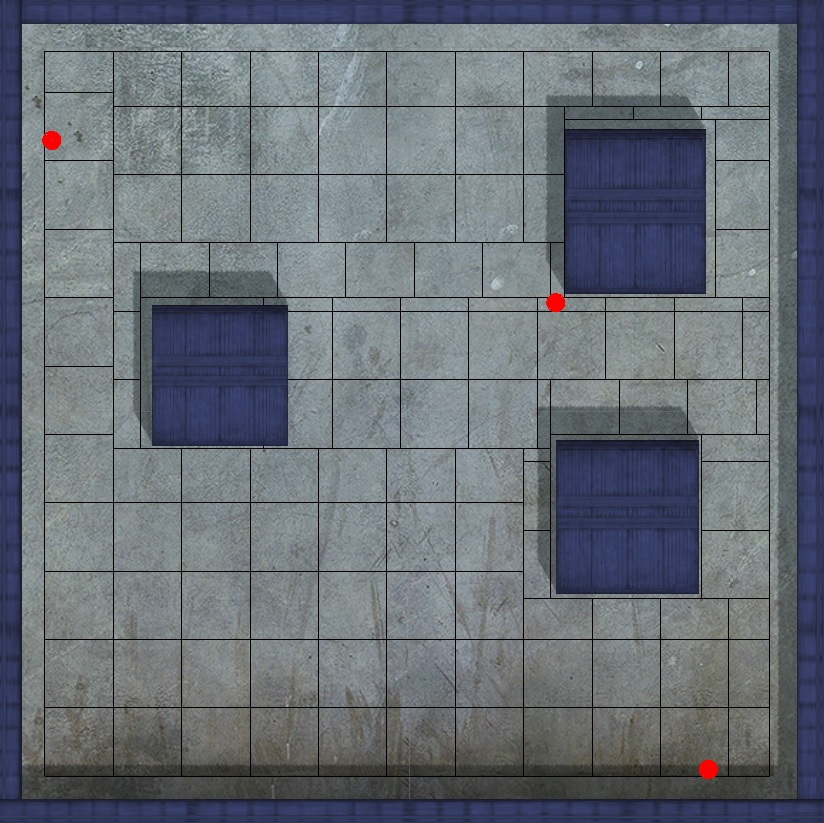
\includegraphics[width=\linewidth,natwidth=824,natheight=823]{fig/staticCoverSet.jpg}
	\end{center}
	\caption{Set cover \& Positions for static guarding}
	\label{staticCoverSet}
\end{figure}